\setcounter{chapter}{6}

\chapter{向量代数与空间解析几何}

\begin{introduction}
    \item 向量的运算
    \item 空间的平面和直线
    \item 空间曲面与空间曲线
\end{introduction}

\section{向量及其运算}
\textbf{向量的数量积(点乘积或内积)}

向量$\bm{a}=\{a_1,a_2,a_3\}$与$\bm{b}=\{b_1,b_2,b_3\}$的数量积是一个数$\left|\bm{a}\right|\cdot\left|\bm{b}\right|\cos\overset{\wedge}{(\bm{a},\bm{b})}$,(且$0\leq \overset{\wedge}{(\bm{a},\bm{b})}\leq \pi$,记作$\bm{a}\cdot\bm{b}$。若向量$\bm{a}$或$\bm{b}$为零向量时,则定义$\bm{a}\cdot\bm{b}=0$,数量积$\bm{a}\cdot\bm{b}$的坐标表示式为
\begin{equation}
    \bm{a}\cdot\bm{b}=a_1 b_1+a_2 b_2+a_3 b_3
    \nonumber
\end{equation}

两个向量$\bm{a},\bm{b}$垂直(或称正交),记作$\bm{a}\perp\bm{b}$,特别地,规定零向量与任意向量垂直。

\begin{property} \label{property:dot_product}
    \begin{enumerate}
        \item $\bm{a}\cdot\bm{b} = \bm{b}\cdot\bm{a}$
        \item $(\lambda \bm{a})\cdot\bm{b} = \lambda(\bm{a}\cdot\bm{b})$
        \item $(\bm{a}+\bm{b})\cdot\bm{c}=\bm{a}\cdot\bm{c}+\bm{b}\cdot\bm{c}$
        \item $\bm{a}\perp\bm{b}$的充分必要条件是$\bm{a}\cdot\bm{b}=0$
    \end{enumerate}
\end{property}
\vspace{2mm}

\textbf{向量的向量积(叉乘积或外积)}

两个向量$\bm{a}$和$\bm{b}$的向量积是一个向量$\bm{c}$,记为$\bm{a}\times\bm{b}$,即$\bm{c}=\bm{a}\times\bm{b}$;$\bm{c}$的模等于$|\bm{a}||\bm{b}|\sin\overset{\wedge}{(\bm{a},\bm{b})}$,$\bm{c}$的方向垂直于$\bm{a}$与$\bm{b}$所决定的平面,且$\bm{a},\bm{b},\bm{c}$顺次构成右手系,若向量$\bm{a}$或$\bm{b}$为零向量时,则定义$\bm{a}\times\bm{b}=0$,向量积$\bm{a}\times\bm{b}$坐标表示式为:
\begin{equation} 
    \bm{a}\times\bm{b}=
    \begin{vmatrix}
        \bm{i} & \bm{j} & \bm{k} \\
        a_1 & a_2 & a_3 \\
        b_1 & b_2 & b_3
    \end{vmatrix}
    = \left\{
        \begin{vmatrix}
            a_2 & a_3 \\
            b_2 & b_3
        \end{vmatrix},
        -\begin{vmatrix}
            a_1 & a_3 \\
            b_1 & b_3
        \end{vmatrix},
        \begin{vmatrix}
            a_1 & a_2 \\
            b_1 & b_2
        \end{vmatrix}
    \right\}
    \nonumber
\end{equation}

\begin{property} \label{property:cross_product}
    \begin{enumerate}
        \item $\bm{a}\times\bm{b} = -\bm{b}\times\bm{a}$
        \item $(\lambda \bm{a})\times\bm{b} = \lambda(\bm{a}\times\bm{b})$
        \item $(\bm{a}+\bm{b})\times\bm{c}=\bm{a}\times\bm{c}+\bm{b}\times\bm{c}$
        \item $\bm{a}\pll\bm{b}$的充分必要条件是$\bm{a}\times\bm{b}=0$
    \end{enumerate}
\end{property}
\vspace{2mm}

\textbf{向量的混合积}

设$\bm{a}=\{a_1,a_2,a_3\},\bm{b}=\{b_1,b_2,b_3\},\bm{c}=\{c_1,c_2,c_3\}$,则称乘积$(\bm{a}\times\bm{b})\cdot\bm{c}$为向量$\bm{a},\bm{b},\bm{c}$的混合积,记为$[\bm{a},\bm{b},\bm{c}]$。

混合积是一数量,其几何意义为:混合积的绝对值等于以$\bm{a},\bm{b},\bm{c}$为相邻三条棱的平行六面体的体积。因此,向量$\bm{a},\bm{b},\bm{c}$共面的充分必要条件是\quad $(\bm{a}\times\bm{b})\cdot\bm{c}=0$

混合积$(\bm{a}\times\bm{b})\cdot\bm{c}$的坐标表达式为
\begin{equation}
    (\bm{a}\times\bm{b})\cdot\bm{c}=
    \begin{vmatrix}
        a_1 & a_2 & a_3 \\
        b_1 & b_2 & b_3 \\
        c_1 & c_2 & c_3
    \end{vmatrix}
    \nonumber
\end{equation}

且
\begin{equation}
    (\bm{a}\times\bm{b})\cdot\bm{c}=(\bm{b}\times\bm{c})\cdot\bm{a}=(\bm{c}\times\bm{a})\cdot\bm{b}
    \nonumber
\end{equation}

\begin{note}
本节的内容可以用行列式的性质去理解记忆
\end{note}

\section{空间的平面和直线}
\textbf{1.平面及其方程}

法向量 \quad 与平面垂直的任意非零向量,称为该平面的法向量.

(1)点法式方程 \quad 设平面过点$M_0(x_0,y_0,z_0)$,其法向量为$\bm{n}=\{A,B,C\}$,则此平面方程为
\begin{equation}
    A(x-x_0)+B(y-y_0)+C(z-z_0)=0
    \nonumber
\end{equation}

(2)截距式方程 \quad 设$a,b,c$分别为平面在$x,y,z$轴上的截距,则此平面方程为
\begin{equation}
    \frac{x}{a}+\frac{y}{b}+\frac{z}{c}=1
    \nonumber
\end{equation}

(3)三点式方程 \quad 设平面过不共线的三点$A(x_1,y_1,z_1),B(x_2,y_2,z_2),C(x_3,y_3,z_3)$,则此平面方程为
\begin{equation}
    \begin{vmatrix}
        x-x_1 & y-y_1 & z-z_1 \\
        x_2-x_1 & y_2-y_1 & z_2-z_1 \\
        x_3-x_1 & y_3-y_1 & z_3-z_1
    \end{vmatrix}=0
    \nonumber
\end{equation}

(4)一般式方程 \quad 平面的一般式方程是三元一次方程
\begin{equation}
    Ax+By+Cz+D=0
    \nonumber
\end{equation}
其中$A,B,C$不同时为零.

\textbf{2.空间直线及其方程}

方向向量 \quad 与直线平行的非零向量,称为该直线的方向向量.

(1)对称式方程(又称点向式或标准式方程)

过点$M_0(x_0,y_0,z_0)$,方向向量为$\bm{s}=\{l,m,n\}$的直线的标准式方程为
\begin{equation}
    \frac{x-x_0}{l}=\frac{y-y_0}{m}=\frac{z-z_0}{n}
    \nonumber
\end{equation}

(2)参数方程 \quad 由标准式方程
\begin{equation}
    \frac{x-x_0}{l}=\frac{y-y_0}{m}=\frac{z-z_0}{n}=t
    \nonumber
\end{equation}
易得直线的参数方程
\begin{equation}
    \begin{cases}
    x=x_0+lt \\
    y=y_0+mt \\
    z=z_0+nt
    \end{cases}
    \quad (t\mbox{为参数})
    \nonumber
\end{equation}

(3)两点式方程 \quad 过点$M_1(x_1,y_1,z_1),M_2(x_2,y_2,z_2)$的直线方程为
\begin{equation}
    \frac{x-x_1}{x_2-x_1}=\frac{y-y_1}{y_2-y_1}=\frac{z-z_1}{z_2-z_1}
    \nonumber
\end{equation}

(4)一般式方程 \quad 直线的一般式方程是三元一次方程
\begin{equation}
    \begin{cases}
    A_1x+B_1y+C_1z+D_1=0 \\
    A_2x+B_2y+C_2z+D_2=0
    \end{cases}
    \nonumber
\end{equation}
其中每一个三元一次方程都表示一个平面.

\textbf{3.直线、平面之间的相对位置关系}

设平面 \quad $\pi_1:A_1x+B_1y+C_1z+D_1=0 \quad \pi_2:A_2x+B_2y+C_2z+D_2=0$,它们的法向量分别为$\bm{n}_1=\{A_1,B_1,C_1\},\bm{n}_2=\{A_2,B_2,C_2\}$

直线 \quad $L_1:\dfrac{x-x_1}{l_1}=\dfrac{y-y_1}{m_1}=\dfrac{z-z_1}{n_1} \quad L_2:\dfrac{x-x_2}{l_2}=\dfrac{y-y_2}{m_2}=\dfrac{z-z_2}{n_2}$,它们的方向向量分别为$\bm{s}_1=\{l_1,m_1,n_1\},\bm{s}_2=\{l_2,m_2,n_2\}$

(1)夹角

平面$\pi_1$与$\pi_2$的夹角$\theta$定义为法向量$\bm{n}_1,\bm{n}_2$的夹角,即
\begin{equation}
    \cos\theta=\dfrac{\bm{n}_1\cdot\bm{n}_2}{|\bm{n}_1|\cdot|\bm{n}_2|}=\dfrac{|A_1A_2+B_1B_2+C_1C_2|}{\sqrt{A_1^2+B_1^2+C_1^2}\cdot\sqrt{A_2^2+B_2^2+C_2^2}}
    \nonumber
\end{equation}

直线$L_1$与$L_2$的夹角$\theta$定义为方向向量$\bm{s}_1,\bm{s}_2$的夹角,即
\begin{equation}
    \cos\theta=\dfrac{\bm{s}_1\cdot\bm{s}_2}{|\bm{s}_1|\cdot|\bm{s}_2|}=\dfrac{|l_1l_2+m_1m_2+n_1n_2|}{\sqrt{l_1^2+m_1^2+n_1^2}\cdot\sqrt{l_2^2+m_2^2+n_2^2}}
    \nonumber
\end{equation}

直线$L_1$与平面$\pi_1$的夹角$\theta$定义为直线$L_1$和它在平面$\pi_1$上的投影所成的两邻角中的锐角,即
\begin{equation}
    \sin\theta=\dfrac{|\bm{s}_1\cdot\bm{n}_1|}{|\bm{s}_1|\cdot|\bm{n}_1|}=\dfrac{|A_1l_1+B_1m_1+C_1n_1|}{\sqrt{A_1^2+B_1^2+C_1^2}\cdot\sqrt{l_1^2+m_1^2+n_1^2}}
    \nonumber
\end{equation}

(2)平行的条件

平面$\pi_1$与$\pi_2$平行的充分必要条件是$\dfrac{A_1}{A_2}=\dfrac{B_1}{B_2}=\dfrac{C_1}{C_2}$

直线$L_1$与$L_2$平行的充分必要条件是$\dfrac{l_1}{l_2}=\dfrac{m_1}{m_2}=\dfrac{n_1}{n_2}$

直线$L_1$与平面$\pi_1$平行的充分必要条件是$l_1A_1+m_1B_1+n_1C_1=0$

(3)垂直的条件

平面$\pi_1$与$\pi_2$垂直的充分必要条件是$A_1A_2+B_1B_2+C_1C_2=0$

直线$L_1$与$L_2$垂直的充分必要条件是$l_1l_2+m_1m_2+n_1n_2=0$

直线$L_1$垂直于平面$\pi_1$的充分必要条件是$\dfrac{l_1}{A_1}=\dfrac{m_1}{B_1}=\dfrac{n_1}{C_1}$

\textbf{4.距离公式}

(1)点到平面的距离

点$M_0(x_0,y_0,z_0)$到平面$Ax+By+Cz+D=0$的距离为$d=\dfrac{|Ax_0+By_0+Cz_0+D|}{\sqrt{A^2+B^2+C^2}}$

(2)点到直线的距离

点$P_1(x_1,y_1,z_1)$到直线$\dfrac{x-x_0}{l}=\dfrac{y-y_0}{m}=\dfrac{z-z_0}{n}$的距离为$d=\dfrac{|\overrightarrow{M_0P_1}\times\bm{s}|}{|\bm{s}|}$,其中,
\begin{equation}
    M_0(x_0,y_0,z_0), \quad \bm{s}=\{l,m,n\}
    \nonumber
\end{equation}

(3)两直线共面的条件

设有两直线 \quad $L_1:\dfrac{x-x_1}{l_1}=\dfrac{y-y_1}{m_1}=\dfrac{z-z_1}{n_1}, \quad L_2:\dfrac{x-x_2}{l_2}=\dfrac{y-y_2}{m_2}=\dfrac{z-z_2}{n_2}$,共面的条件为$\overrightarrow{P_1P_2}\cdot(\bm{a}\times\bm{b})=0$,其中
\begin{equation}
    P_1(x_1,y_1,z_1), \quad P_2(x_2,y_2,z_2), \quad \bm{a}=\{l_1,m_1,n_1\}, \quad \bm{b}=\{l_2,m_2,n_2\}
\end{equation}

(4)两直线间的距离

两异面直线$L_1,L_2$的距离为$d=\dfrac{|\overrightarrow{P_1P_2}\cdot(\bm{a}\times\bm{b})|}{|\bm{a}\times\bm{b}|}$

\section{空间曲面与空间曲线}
\textbf{1.空间曲面方程}

(1)一般方程 $F(x,y,z)=0$

(2)显式方程 $z=f(x,y)$

(3)参数方程 $\left\{\begin{aligned}& x=x(u,v) \\ & y=y(u,v) \\ & z=z(u,v) \end{aligned}\right.$ \quad $(u,v)\in D$,其中$D$为$uv$平面上某一区域

\textbf{2.旋转曲面方程}

设$C:f(y,z)=0$为$yOz$平面上的曲线,则

(1)$C$绕$z$轴旋转所得的曲面为$f(\pm\sqrt{x^2+y^2},z)=0$

(2)$C$绕$y$轴旋转所得的曲面为$f(x,\pm\sqrt{y^2+z^2})=0$

旋转曲面主要由母线和旋转轴确定.

求旋转曲面方程时,平面曲线绕某坐标轴旋转,则该坐标轴对应的变量不变,而曲线方程中另一变量改写成该变量与第三变量平方和的正负平方根,例如:$L\left\{\begin{aligned}& f(x,y)=0 \\ & z=0 \end{aligned}\right.$.曲线$L$绕$x$轴旋转所形成的旋转曲面的方程为$f(x,\pm\sqrt{y^2+z^2})=0$

\textbf{3.柱面方程}

(1)母线平行于$z$轴的柱面方程为$F(x,y)=0$

(2)母线平行于$x$轴的柱面方程为$G(y,z)=0$

(3)母线平行于$y$轴的柱面方程为$H(x,z)=0$

当曲面方程中缺少一个变量时,则曲面为柱面,如$F(x,y)=0$,变量$z$未出现,该曲面表示由准线$\left\{\begin{aligned}& F(x,y)=0 \\ & z=0 \end{aligned}\right.$生成,母线平行于$z$轴的柱面.

柱面方程必须注意准线与母线两个要素

\newpage
\addcontentsline{toc}{section}{Problem Plus}
\section*{Problem Plus}
\begin{note}
    以下内容需要一定线性代数知识基础
\end{note}

你是否思考过一个问题,即为什么形如$Ax+By+Cz+D=0$这样的表达式表示出来的是一个平面?

我们举一个简单的例子,假设一个平面为$x+y+z=0$,那么可以将这个平面式拆分为矩阵形式:
\begin{equation}
    \begin{bmatrix}
        1 & 1 & 1
    \end{bmatrix}
    \begin{bmatrix}
        x \\ y \\ z
    \end{bmatrix}
    =0
    \nonumber
\end{equation}

而$x+y+z=0$这个平面实际上是$\begin{bmatrix} 1 & 1 & 1 \end{bmatrix}$的零空间(Nullspace),即我们现在将上式抽象为矩阵方程$\mathbf{A}\mathbf{x}=0$,所谓零空间,即可理解为这个系数矩阵所对应的基础解系张成(span)的空间。让我们接着往下:

因为$\begin{bmatrix} 1 & 1 & 1 \end{bmatrix}$已经是行最简阶梯形(Row Reduced Echelon Form),所以易得一个基础解系
\begin{equation*}
    \mathbf{x}=c_1\begin{bmatrix} -1 \\ 1 \\ 0 \end{bmatrix} + c_2\begin{bmatrix} -1 \\ 0 \\ 1 \end{bmatrix} \quad (c_1, c_2 \in \mathbb{R}).
\end{equation*}

细心的你可能会发现,在这个等式中,$\text{rank}(\mathbf{A})=1, \text{rank}(\mathbf{x})=2$,同时可以观察到一个规律,对于任何矩阵等式$\mathbf{Ax}=0$,都有$\text{rank}(\mathbf{A})+\text{rank}(\mathbf{x})\leq \text{the number of A's columns}$,而这两个秩所对应的两个空间,正是$\mathbf{A}$的列空间(column space)和$\mathbf{x}$的零空间(nullspace)。而这个零空间的两个向量张出来的面即为平面$x+y+z=0$。

\begin{figure}[H]
    \centering
    \centerline{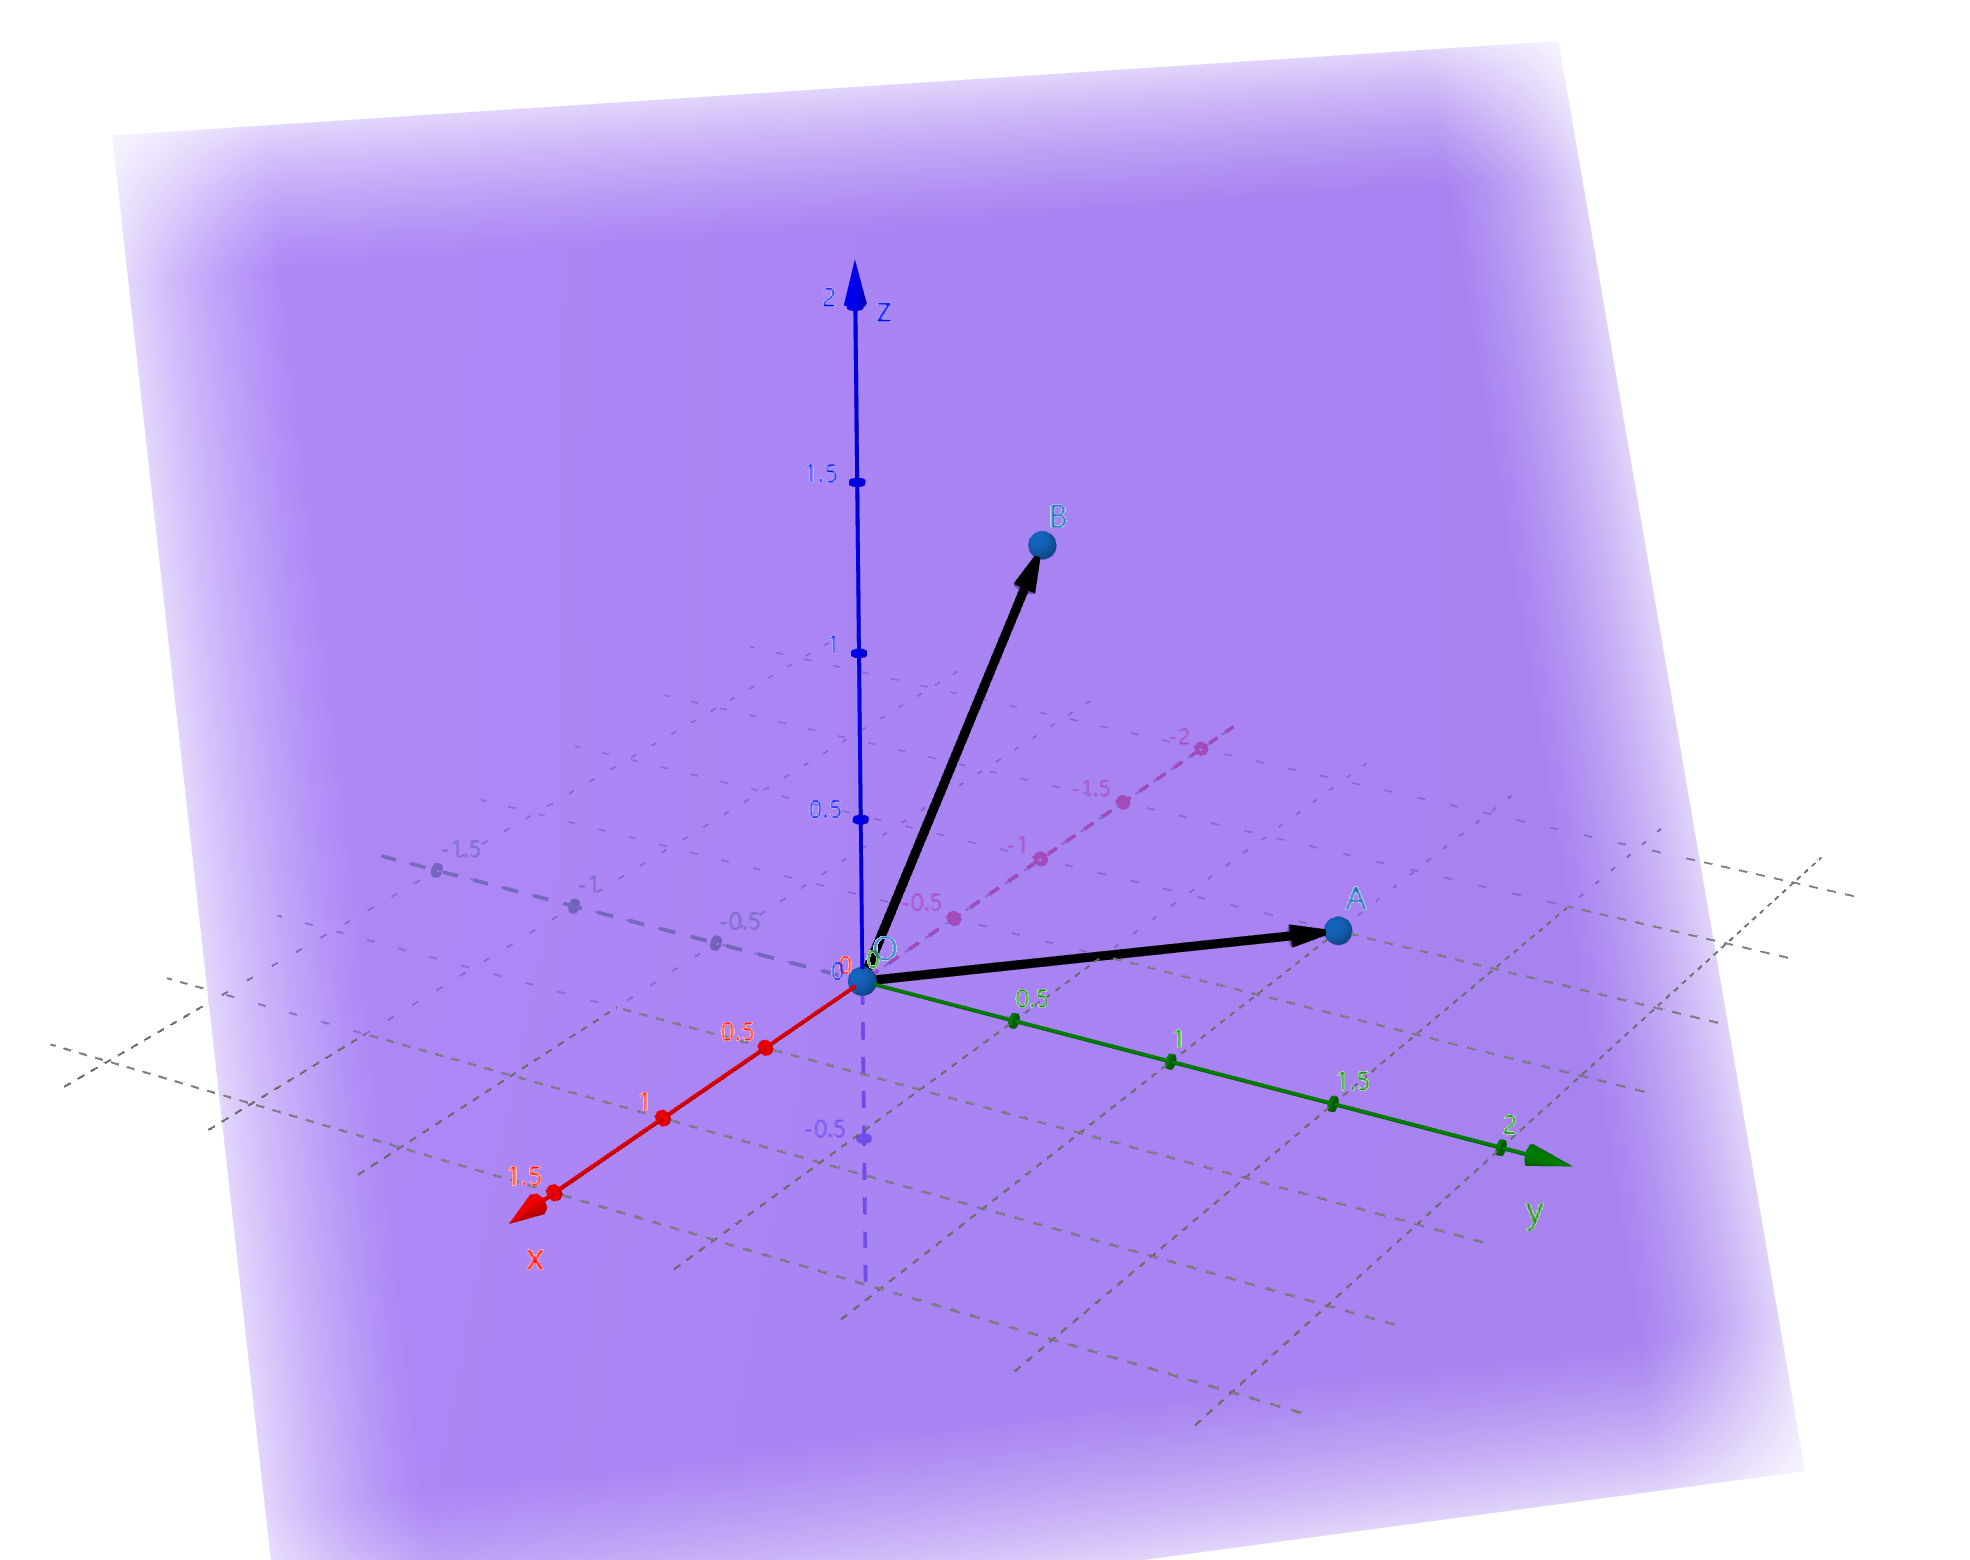
\includegraphics[width=12cm]{figure/nullspace_for_2d_plane.png}}
    \caption{矩阵的零空间张出的平面表示} \label{nullspace}
\end{figure}

基于这个思考方式,我们也可以理解平面束为何可以表示一条直线,这里就不过多赘述了,留给读者思考。